\section{Cấu tạo bảng tuần hoàn các nguyên tố hóa học}
\begin{Muctieu}
	\begin{itemize}
		\item  Nêu được lịch sử phát minh định luật tuần hoàn và bảng tuần hoàn các nguyên tố hoá học.
		\item  Mô tả được cấu tạo của bảng tuần hoàn các nguyên tố hoá học và nêu được các khái niệm liên quan: ô, chu kì, nhóm.
		\item  Nêu được nguyên tắc sắp xếp của bảng tuần hoàn các nguyên tố hoá học.
		\item  Phân loại được nguyên tố hóa học.
	\end{itemize}
\end{Muctieu}
\begin{kd}
	Các em có bao giờ tự hỏi làm thế nào các nhà khoa học có thể sắp xếp hơn 100 nguyên tố hóa học một cách có trật tự không?
	Bảng tuần hoàn là một công cụ quan trọng trong hóa học, giúp chúng ta hiểu và dự đoán tính chất của các nguyên tố. Nó không chỉ đơn giản là một danh sách các nguyên tố, mà còn cho chúng ta biết rất nhiều thông tin về cấu trúc và đặc tính của chúng.
\end{kd}
\subsection{NỘI DUNG BÀI HỌC}
	\subsubsection{Lịch sử phát minh bảng tuần hoàn}
\begin{longtable}{>{\raggedright\arraybackslash}p{0.18\textwidth}>{\raggedright\arraybackslash}p{0.28\textwidth}>{\raggedright\arraybackslash}p{0.23\textwidth}>{\raggedright\arraybackslash}p{0.23\textwidth}}
	\caption{Lịch sử phát triển bảng hệ thống tuần hoàn các nguyên tố hóa học} \\
	\toprule \rowcolor{\mycolor!20}
	\indam{Giai đoạn} & \indam{Nội dung chính} & \indam{Ưu điểm} & \indam{Hạn chế} \\
	\midrule
	\endfirsthead
	\multicolumn{4}{c}{%
		{\bfseries \tablename\ \thetable{} -- tiếp theo}} \\
	\toprule\rowcolor{\mycolor!20}
	\indam{Giai đoạn} & \indam{Nội dung chính} & \indam{Ưu điểm} & \indam{Hạn chế} \\
	\midrule
	\endhead
	\endfoot
	\bottomrule
	\endlastfoot
	\rowcolor{\mauphu!10}
	\multirow{3}{=}{\textbf{Thời kỳ đầu (trước 1800)}} & 
	\begin{myitemize}
		\item Phân loại nguyên tố theo tính chất
		\item Antoine Lavoisier (1789) công bố 33 nguyên tố
	\end{myitemize} & 
	\begin{myitemize}
		\item Bước đầu hệ thống hóa kiến thức
		\item Xác định được các nguyên tố cơ bản
	\end{myitemize} & 
	\begin{myitemize}
		\item Chưa có hệ thống phân loại rõ ràng
		\item Số lượng nguyên tố còn hạn chế
	\end{myitemize} \\ 
	\midrule
	\rowcolor{\mycolor!10}
	\multirow{3}{=}{\textbf{Thập niên 1820-1830}} & 
	Johann Döbereiner (1829) phát hiện quy luật bộ ba & 
	\begin{myitemize}
		\item Phát hiện mối liên hệ giữa các nguyên tố
		\item Gợi ý về tính tuần hoàn
	\end{myitemize} & 
	Chỉ áp dụng được cho một số bộ ba nguyên tố \\ 
	\midrule
	\rowcolor{\mauphu!10}
	\multirow{4}{=}{\textbf{Thập niên 1860}} & 
	\begin{myitemize}
		\item John Newlands (1863): Quy luật bát âm
		\item Lothar Meyer và Dmitri Mendeleev (1869): Bảng tuần hoàn đầu tiên
	\end{myitemize} & 
	\begin{myitemize}
		\item Xác định được tính tuần hoàn
		\item Đặt nền móng cho bảng tuần hoàn hiện đại
	\end{myitemize} & 
	Quy luật bát âm không áp dụng được cho tất cả nguyên tố \\
	\midrule
	\rowcolor{\mycolor!10}
	\multirow{3}{=}{\textbf{Bảng tuần hoàn của Mendeleev (1869)}}
	& 
	\begin{myitemize}
		\item Sắp xếp 63 nguyên tố theo khối lượng nguyên tử
		\item Dự đoán nguyên tố chưa phát hiện
	\end{myitemize} & 
	\begin{myitemize}
		\item Dự đoán chính xác các nguyên tố mới
		\item Cơ sở cho bảng tuần hoàn hiện đại
	\end{myitemize} & 
	Một số vị trí sắp xếp chưa chính xác do dựa vào khối lượng nguyên tử \\
	\midrule
	\rowcolor{\mauphu!10}
	\multirow{4}{=}{\textbf{Thế kỷ 20}} & 
	\begin{myitemize}
		\item Henry Moseley (1913): Sắp xếp theo số proton
		\item Glenn Seaborg (1940s): Thêm actinide
	\end{myitemize} & 
	\begin{myitemize}
		\item Sắp xếp chính xác hơn dựa trên cấu trúc nguyên tử
		\item Mở rộng bảng với các nguyên tố nặng
	\end{myitemize} & 
	Khó khăn trong việc tổng hợp và nghiên cứu các nguyên tố siêu nặng \\
	\midrule
	\rowcolor{\mycolor!10}
	\multirow{4}{=}{\textbf{Hiện đại}} & 
	\begin{myitemize}
		\item 118 nguyên tố được IUPAC công nhận
		\item Nghiên cứu nguyên tố siêu nặng
	\end{myitemize} & 
	\begin{myitemize}
		\item Bảng tuần hoàn hoàn chỉnh và chuẩn hóa
		\item Tiếp tục mở rộng kiến thức về các nguyên tố mới
	\end{myitemize} & 
	Thách thức trong việc tổng hợp và xác định tính chất của các nguyên tố siêu nặng \\
\end{longtable}
\subsubsection{Nguyên tắc sắp xếp của bảng tuần hoàn các nguyên tố hóa học}
\begin{tomtat}
	\begin{itemize}
		\item  Các nguyên tố hoá học được sắp xếp từ trái sang phải và từ trên xuống dưới theo chiều tăng dần điện tích hạt nhân của nguyên từ.
		\item  Các nguyên tố mà nguyên tử có cùng số lớp electron được xếp vào cùng một hàng.
		\item  Các nguyên tố mà nguyên từ có số electron hoá trị\footnotemark[1]  như nhau được xếp vào củng một cột.
	\end{itemize}
\end{tomtat}
\footnotetext[1]{Electron hoá trị là những electron có khả năng tham gia vào việc hình thành liên kết hoá học (thường là những electron ở lớp ngoài cùng).}
\subsubsection{Cấu tạo bảng tuần hoàn}
\Noibat[\maunhan][][\faArrowCircleORight][]{Tìm hiểu về ô nguyên tố}
\begin{paracol}{2}
	\tikz[node distance=1mm] {
		\path (0,0) node[anchor =center](be){
			\nguyento[color=\mauphu,show notes=true]{4}{9.012}{Be}{Beryllium}{$[He] 2s^2$}{+2}};
	}
	\captionof{figure}{Ô nguyên tố Beryllium\label{fig:Be elemnt}}
	\switchcolumn
	\begin{hoivadap}
		\begin{cauhoi}
			Quan sát hình (\ref{fig:Be elemnt}) hãy cho biết các thông tin có trong nguyên tố Beryllium
		\end{cauhoi}
	\end{hoivadap}
\end{paracol}
\begin{ghinho}
	\indam{Ô nguyên tố.} Mỗi nguyên tố hoá học được xếp vào một ô trong bảng tuần hoàn, gọi là ô nguyên tố. Mỗi ô chứa một số thông tin của một nguyên tố hoá học như. kí hiệu hoá học, tên nguyên tố, số hiệu nguyên tử và nguyên tử khối trung bình,$\ldots$
	\begin{center}
		\boxct{\indam{Số thứ tự ô nguyên tố = số hiệu nguyên tử}}
	\end{center}
\end{ghinho}
\Noibat[\maunhan][][\faArrowCircleORight][]{Tìm hiểu về chu kì}

\resizebox{0.9\linewidth}{!}{
	%%CK2
	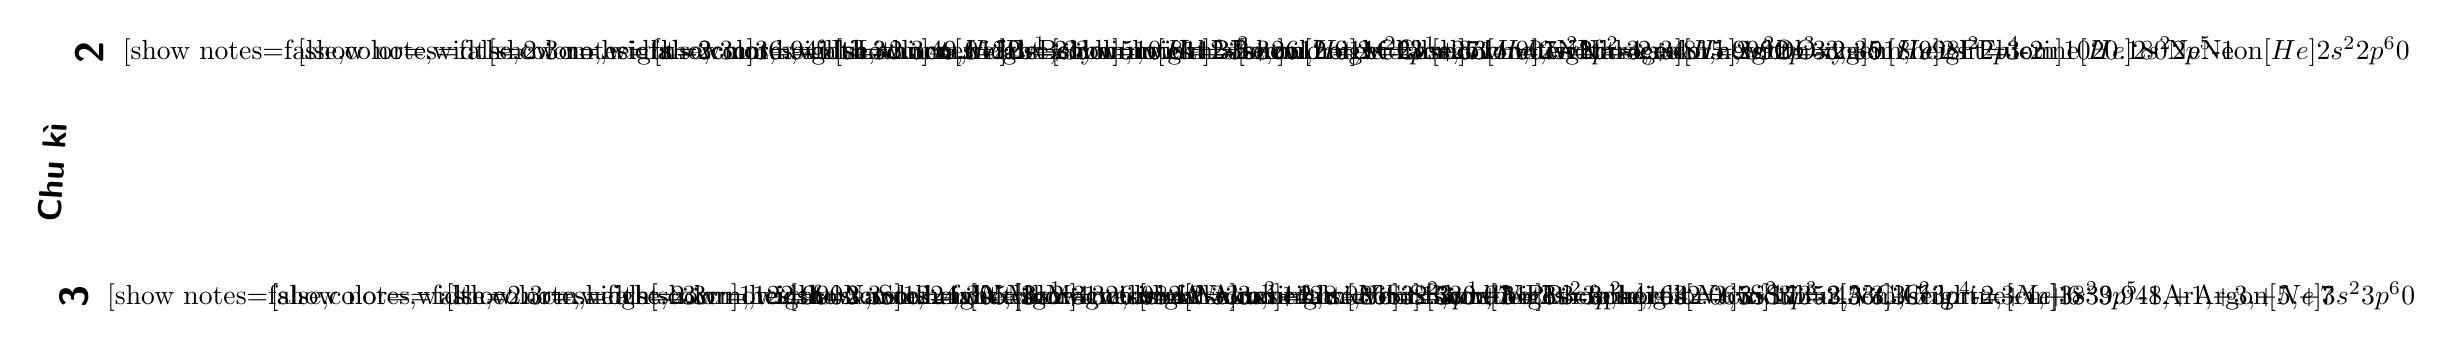
\begin{tikzpicture}[node distance=1mm]
		\foreach \num/\mass/\sym/\name/\config/\ox [count=\i from 1] in {
			3/6.941/Li/Lithium/$[He] 2s^1$/+1,
			4/9.012/Be/Beryllium/$[He] 2s^2$/+2,
			5/10.811/B/Boron/$[He]2s^2 2p^1$/+3,
			6/12.011/C/Carbon/$[He]2s^2 2p^2$/\text{-4,+4},
			7/14.007/N/Nitrogen/$[He]2s^2 2p^3$/\text{-3,+5},
			8/15.999/O/Oxygen/$[He]2s^2 2p^4$/-2,
			9/18.998/F/Fluorine/$[He]2s^2 2p^5$/-1,
			10/20.180/Ne/Neon/$[He]2s^2 2p^6$/0
		} {
			\path (\i*2.4cm,0) node[anchor=center] (element-2-\i) {
				\nguyento[show notes=false,color=\mauphu,width=2.3cm,height=3cm]{\num}{\mass}{\sym}{\name}{\config}{\ox}
			};
		}
		%%CK3
		\foreach \num/\mass/\sym/\name/\config/\ox [count=\i from 1] in {
			11/22.990/Na/Sodium/$[Ne] 3s^1$/+1,
			12/24.305/Mg/Magnesium/$[Ne] 3s^2$/+2,
			13/26.982/Al/Aluminium/$[Ne] 3s^2 3p^1$/+3,
			14/28.086/Si/Silicon/$[Ne] 3s^2 3p^2$/\text{-4,+4},
			15/30.974/P/Phosphorus/$[Ne] 3s^2 3p^3$/\text{-3,+3,+5},
			16/32.065/S/Sulfur/$[Ne] 3s^2 3p^4$/\text{-2,+4,+6},
			17/35.453/Cl/Chlorine/$[Ne]3s^23p^5$/\text{-1,+1,+3,+5,+7},
			18/39.948/Ar/Argon/$[Ne]3s^23p^6$/0
		} {
			\path (\i*2.4cm,-3.1cm) node[anchor=center] (element-3-\i) {
				\nguyento[show notes=false,color=\maunhan,width=2.3cm,height=3cm]{\num}{\mass}{\sym}{\name}{\config}{\ox}
			};
		}
		%%Thông tin chu kì
		\path (element-2-1.south west)--(element-2-1.north west) node[sloped,above,font=\Large\bfseries\sffamily,pos=0.5] (ck2){2};
		\path (element-3-1.south west)--(element-3-1.north west) node[sloped,above,font=\Large\bfseries\sffamily,pos=0.5] (ck3){3};
		\path (ck3)--(ck2) node[sloped,above=3pt,font=\large\bfseries\sffamily,pos=0.5] {Chu kì};
	\end{tikzpicture}
}
\captionof{figure}{Các nguyên tố thuộc chu kì 2 và chu kì 3 \label{fig:ck-2-3}}

\begin{hoivadap}
	\begin{cauhoi}
		Quan sát hình (\ref{fig:ck-2-3}) hãy cho biết số lớp electron các nguyên tố thuộc cùng chu kì
	\end{cauhoi}
\end{hoivadap}

\begin{ghinho}
	\indam{Chu kì} là tập hợp các nguyên tố có cùng số lớp electron.\\
	Bảng tuần hoàn có 7 chu kì:
	\begin{itemize}
		\item Chu kì 1,2,3 là chu kì nhỏ
		\item Chu kì 4,5,6,7 là chu kì lớn
	\end{itemize}
	\begin{center}
		\boxct{\indam{Số thứ tự chu kì = số lớp electron}}
	\end{center}
\end{ghinho}
\Noibat[\maunhan][][\faArrowCircleORight][]{Tìm hiểu về nhóm}
\begin{ghinho}
	\indam{Nhóm} là tập hợp các nguyên tố mà nguyên tử có cấu hình electron tương tự nhau (trừ nhóm VIIIB), do đó có tính chất hoá học gần giống nhau và được xếp theo cột.
	\begin{center}
		\boxct{\indam{Số thứ tự của nhóm A = số electron ở lớp ngoài cùng }}
	\end{center}
\end{ghinho}
\Noibat[\maunhan][][\faArrowCircleORight][]{Phân loại nguyên tố}
\begin{tomtat}
	Các nguyên tố hoá học cũng có thể được chia thành các khối như sau:
	\begin{itemize}
		\item  Khối các nguyên tố s gồm các nguyên tố thuộc nhóm IA và nhóm IIA, có cấu hình electron: [Khí hiếm] ns $\mathrm{s}^{1+2}$
		\item  Khối các nguyên tố p gồm các nguyên tố thuộc nhóm IIIA đến nhóm VIIIA (trừ nguyên tố He ), có cấu hình electron: [Khí hiếm] $\mathrm{ns}^2 \mathrm{np}^{1+6}$.
		\item  Khối các nguyên tố d gồm các nguyên tố thuộc nhóm B , có cấu hình electron: $\left[\right.$ Khí hiếm] $(\mathrm{n}-1) \mathrm{d}^{1+10} \mathrm{~ns}^{1+2}$.
		\item  Khối các nguyên tố f gồm các nguyên tố xếp thành hai hàng ở cuối bảng tuần hoàn, có cấu hình electron: [Khí hiếm] $(\mathrm{n}-2) \mathrm{f}^{0+14}(\mathrm{n}-1) \mathrm{d}^{0-2} \mathrm{~ns}$ (trong đó $\mathrm{n}=6$ và $\mathrm{n}=7$ ). Chúng gồm 14 nguyên tố họ Lanthanide (từ Ce đến Lu ) và 14 nguyên tố họ Actinide (từ Th đến Lr ).
	\end{itemize}
\end{tomtat}
\Noibat[\maunhan][\myfont[16]{qag}][\faArrowCircleORight][]{Nguyên tắc sắp xếp các nguyên tố trong bảng tuần hoàn}
\begin{tongket}{Ghi nhớ}
	\begin{enumerate}
		\item Các nguyên tố được xếp theo chiều tăng dần của điện tích hạt nhân nguyên tử.
		\item Các nguyên tố có cùng số lớp electron trong nguyên tử được xếp cùng một chu kì.
		\item Các nguyên tố có cùng số electron hoá trị trong nguyên tử được xếp cùng một nhóm, trừ nhóm VIIIB.
	\end{enumerate}
\end{tongket}
\subsection{Các dạng bài tập}
	%%%%================Dạng 1=========================%%%
\begin{dang}{Lý thuyết về cấu tạo bảng tuần hoàn}\end{dang}
\begin{pp}
	Nắm vững một số nội dung chính , ưu điểm và hạn chế về các giai đoạn phát triển bảng hệ thống tuần hoàn.
\end{pp}
%%%Ví dụ mẫu dạng 1%%%
\Noibat[\maunhan][][\faBookmark]{Ví dụ mẫu}
%%%=============VDM 1=============%%%
\begin{vdex}
	Quy luật bộ ba của Döbereiner (1829) có ưu điểm nào sau đây?
	\choice
	{Sắp xếp được tất cả các nguyên tố đã biết}
	{Dự đoán được sự tồn tại của các nguyên tố mới}
	{\True Chỉ ra mối liên hệ giữa khối lượng nguyên tử và tính chất của nguyên tố}
	{Sắp xếp nguyên tố theo số nguyên tử tăng dần}
	\loigiai{
		Quy luật bộ ba của Döbereiner chỉ ra rằng khối lượng nguyên tử của nguyên tố ở giữa xấp xỉ bằng trung bình cộng khối lượng nguyên tử của hai nguyên tố ở hai đầu. Điều này lần đầu tiên cho thấy mối liên hệ giữa khối lượng nguyên tử và tính chất của nguyên tố. Tuy nhiên, quy luật này chỉ áp dụng được cho một số bộ ba nguyên tố, không phải tất cả các nguyên tố đã biết.
	}
\end{vdex}
%%%=============VDM 2=============%%%
\begin{vdex}
	Các nguyên tố có đặc điểm như thế nào thì được xếp vào cùng một hàng (chu kỳ) trong bảng tuần hoàn?
	\choice
	{Có cùng số proton}
	{Có cùng số electron hóa trị}
	{\True Có cùng số lớp electron}
	{Có cùng số neutron}
	\loigiai{
		Các nguyên tố được xếp vào cùng một hàng (chu kỳ) trong bảng tuần hoàn khi chúng có cùng số lớp electron. Số lớp electron quyết định vị trí của nguyên tố trong chu kỳ, và các nguyên tố trong cùng chu kỳ có cùng số lớp electron.
	}
\end{vdex}
\Noibat[][][\faBank]{Bài tập tự luyện dạng \thedang}
\phan{Câu hỏi trắc nghiệm 1 phương án}
\Opensolutionfile{ansex}[Ans/LGEX-Hoa10_C02_CTBTH_BTTL01]
\Opensolutionfile{ans}[Ans/Ans-Hoa10_C02_CTBTH_BTTL01]
%\tatloigiaiex
%\luuloigiaiex
%%%=============EX_1=============%%%
\begin{ex}%[0H2H1-1]
	Nhược điểm chính của Quy luật bát âm của Newlands (1863) là gì?
	\choice
	{Không dự đoán được sự tồn tại của nguyên tố mới}
	{\True Chỉ áp dụng được cho 20 nguyên tố đầu tiên}
	{Không chỉ ra mối liên hệ giữa khối lượng nguyên tử và tính chất của nguyên tố}
	{Sắp xếp nguyên tố theo số khối tăng dần}
	\loigiai{
		Quy luật bát âm của Newlands chỉ ra rằng khi sắp xếp các nguyên tố theo khối lượng nguyên tử tăng dần, cứ 8 nguyên tố thì tính chất lặp lại. Tuy nhiên, quy luật này chỉ áp dụng được cho 20 nguyên tố đầu tiên. Khi áp dụng cho các nguyên tố nặng hơn, quy luật này không còn chính xác. Đây là nhược điểm chính của phương pháp này.
	}
\end{ex}
%%%=============EX_2=============%%%
\begin{ex}%[0H2H1-1]
	Ưu điểm quan trọng nhất của bảng tuần hoàn Mendeleev (1869) là gì?
	\choice
	{Sắp xếp nguyên tố theo số nguyên tử tăng dần}
	{\True Dự đoán được sự tồn tại và tính chất của các nguyên tố chưa phát hiện}
	{Giải thích được cấu trúc electron của nguyên tố}
	{Áp dụng được cho tất cả các nguyên tố, kể cả các nguyên tố nhân tạo}
	\loigiai{
		Bảng tuần hoàn của Mendeleev có nhiều ưu điểm, nhưng ưu điểm quan trọng nhất là khả năng dự đoán sự tồn tại và tính chất của các nguyên tố chưa phát hiện. Mendeleev để lại các ô trống trong bảng và dự đoán tính chất của các nguyên tố sẽ điền vào đó. Nhiều dự đoán của ông đã được chứng minh là chính xác khi các nguyên tố này được phát hiện sau đó, ví dụ như gallium, germanium và scandium.
	}
\end{ex}
%%%=============EX_3=============%%%
\begin{ex}%[0H2H1-1]
	Phát hiện của Moseley (1913) đã khắc phục được nhược điểm nào của bảng tuần hoàn Mendeleev?
	\choice
	{Không giải thích được sự tồn tại của đồng vị}
	{\True Sự sắp xếp không chính xác của một số cặp nguyên tố (ví dụ: Te và I)}
	{Không dự đoán được sự tồn tại của khí hiếm}
	{Không giải thích được cấu trúc electron của nguyên tố}
	\loigiai{
		Moseley phát hiện ra rằng mỗi nguyên tố có một số nguyên tử đặc trưng, và số này tăng dần khi đi từ nguyên tố này sang nguyên tố khác trong bảng tuần hoàn. Phát hiện này đã giải quyết được vấn đề sắp xếp không chính xác của một số cặp nguyên tố trong bảng Mendeleev, như trường hợp của Telua (Te) và Iod (I). Trong bảng của Mendeleev, Te (khối lượng nguyên tử 127,6) được đặt trước I (khối lượng nguyên tử 126,9) mặc dù có khối lượng nguyên tử lớn hơn. Phát hiện của Moseley cho thấy số nguyên tử của Te (52) nhỏ hơn I (53), giải thích được vị trí đúng của chúng trong bảng tuần hoàn.
	}
\end{ex}
%%%=============EX_4=============%%%
\begin{ex}%[0H2H1-1]
	Ai là người đầu tiên đề xuất quy luật bộ ba trong việc sắp xếp các nguyên tố hóa học?
	\choice
	{Newlands}
	{Mendeleev}
	{\True Döbereiner}
	{Moseley}
	\loigiai{
		Johann Wolfgang Döbereiner là người đầu tiên đề xuất quy luật bộ ba vào năm 1829. Ông nhận thấy rằng trong một số bộ ba nguyên tố có tính chất tương tự, khối lượng nguyên tử của nguyên tố giữa xấp xỉ bằng trung bình cộng khối lượng nguyên tử của hai nguyên tố ở hai đầu.
	}
\end{ex}
%%%=============EX_5=============%%%
\begin{ex}%[0H2H1-1]
	\lq\lq Quy luật bát âm\rq\rq trong lịch sử phát triển bảng tuần hoàn được đề xuất bởi ai?
	\choice
	{Mendeleev}
	{\True Newlands}
	{Döbereiner}
	{Moseley}
	\loigiai{
		John Newlands đề xuất \lq\lq Quy luật bát âm \rq\rq vào năm 1863. Ông nhận thấy rằng khi sắp xếp các nguyên tố theo thứ tự tăng dần của khối lượng nguyên tử, cứ mỗi nguyên tố thứ tám thì có tính chất tương tự với nguyên tố đầu tiên, giống như các nốt nhạc trong âm nhạc.
	}
\end{ex}
%%%=============EX_6=============%%%
\begin{ex}%[0H2H1-1]
	Đóng góp quan trọng nhất của Mendeleev trong việc xây dựng bảng tuần hoàn là gì?
	\choice
	{Sắp xếp nguyên tố theo số nguyên tử tăng dần}
	{\True Để lại các ô trống và dự đoán tính chất của các nguyên tố chưa phát hiện}
	{Phát hiện ra các đồng vị của nguyên tố}
	{Giải thích cấu trúc electron của nguyên tố}
	\loigiai{
		Dmitri Mendeleev đã để lại các ô trống trong bảng tuần hoàn của mình và dự đoán tính chất của các nguyên tố chưa phát hiện. Điều này cho phép ông dự đoán sự tồn tại và tính chất của các nguyên tố như gallium, germanium và scandium, mà sau này đã được phát hiện và chứng minh là chính xác.
	}
\end{ex}
%%%=============EX_7=============%%%
\begin{ex}%[0H2H1-1]
	Phát hiện nào của Moseley đã cải tiến bảng tuần hoàn của Mendeleev?
	\choice
	{Khái niệm về đồng vị}
	{\True Số hiệu nguyên tử đặc trưng cho mỗi nguyên tố}
	{Cấu trúc electron của nguyên tử}
	{Sự tồn tại của các nguyên tố nhân tạo}
	\loigiai{
		Henry Moseley phát hiện ra rằng mỗi nguyên tố có một số nguyên tử đặc trưng, và số này tăng dần khi đi từ nguyên tố này sang nguyên tố khác trong bảng tuần hoàn. Phát hiện này đã giải quyết được vấn đề sắp xếp không chính xác của một số cặp nguyên tố trong bảng Mendeleev và xác định chính xác vị trí của các nguyên tố trong bảng tuần hoàn.
	}
\end{ex}
%%%=============EX_8=============%%%
\begin{ex}%[0H2H1-1]
	Trong bảng tuần hoàn hiện đại, các nguyên tố được sắp xếp theo thứ tự tăng dần của đại lượng nào?
	\choice
	{Khối lượng nguyên tử}
	{\True Số hiệu nguyên tử }
	{Số khối}
	{Số neutron trong hạt nhân}
	\loigiai{
		Trong bảng tuần hoàn hiện đại, các nguyên tố được sắp xếp theo thứ tự tăng dần của số hiệu nguyên tử hay số đơn vị điện tích hạt nhân (= số proton) trong hạt nhân. Điều này dựa trên phát hiện của Moseley và đảm bảo sự sắp xếp chính xác của các nguyên tố.
	}
\end{ex}
%%%=============EX_9=============%%%
\begin{ex}%[0H2N1-1]
	Định nghĩa của \lq\lq chu kỳ \rq\rq trong bảng tuần hoàn là gì?
	\choice
	{Một cột dọc trong bảng tuần hoàn}
	{\True Một hàng ngang trong bảng tuần hoàn, trong đó các nguyên tố có cấu hình electron lớp ngoài cùng biến đổi tuần hoàn}
	{Một nhóm các nguyên tố có tính chất hóa học giống nhau}
	{Khoảng cách giữa hai nguyên tố liên tiếp trong bảng}
	\loigiai{
		Một chu kỳ trong bảng tuần hoàn là một hàng ngang, trong đó các nguyên tố được sắp xếp theo thứ tự tăng dần của số nguyên tử. Trong một chu kỳ, cấu hình electron lớp ngoài cùng của các nguyên tố biến đổi tuần hoàn từ 1 đến 8 electron (trừ chu kỳ 1).
	}
\end{ex}
%%%=============EX_10=============%%%
\begin{ex}%[0H2N1-1]
	\lq\lq Nhóm \rq\rq trong bảng tuần hoàn được định nghĩa như thế nào?
	\choice
	{Một hàng ngang trong bảng tuần hoàn}
	{Các nguyên tố có cùng số khối}
	{\True Một cột dọc chứa các nguyên tố có cấu hình electron lớp ngoài cùng tương tự nhau}
	{Các nguyên tố có cùng số neutron}
	\loigiai{
		Một nhóm trong bảng tuần hoàn là một cột dọc chứa các nguyên tố có cấu hình electron lớp ngoài cùng tương tự nhau. Do đó, các nguyên tố trong cùng một nhóm thường có tính chất hóa học tương tự nhau.
	}
\end{ex}
%%%=============EX_11=============%%%
\begin{ex}%[0H2N1-1]
	Bảng tuần hoàn hiện đại có bao nhiêu chu kỳ?
	\choice
	{6}
	{\True 7}
	{8}
	{18}
	\loigiai{
		Bảng tuần hoàn hiện đại có 7 chu kỳ. Chu kỳ 1 là chu kỳ ngắn nhất với 2 nguyên tố, chu kỳ 2 và 3 có 8 nguyên tố, chu kỳ 4 và 5 có 18 nguyên tố, chu kỳ 6 có 32 nguyên tố, và chu kỳ 7 là chu kỳ chưa hoàn thiện.
	}
\end{ex}
%%%=============EX_12=============%%%
\begin{ex}%[0H2N1-1]
	Bảng tuần hoàn hiện đại có bao nhiêu nhóm?
	\choice
	{8}
	{16}
	{\True 18}
	{32}
	\loigiai{
		Bảng tuần hoàn hiện đại có 18 nhóm. Các nhóm được đánh số từ 1 đến 18, trong đó nhóm 1-2 và 13-18 là các nguyên tố chính, nhóm 3-12 là các nguyên tố chuyển tiếp.
	}
\end{ex}
%%%=============EX_13=============%%%
\begin{ex}%[0H2H1-1]
	Nguyên tố nào sau đây không phải là nguyên tố họ s?
	\choice
	{Lithium}
	{Beryllium}
	{\True Boron}
	{Sodium}
	\loigiai{
		Boron (B) không phải là nguyên tố họ s. Nó là nguyên tố họ p, thuộc nhóm 13 trong bảng tuần hoàn. Các nguyên tố họ s là những nguyên tố có electron cuối cùng điền vào orbital s, bao gồm các nguyên tố ở nhóm 1 (trừ H) và nhóm 2.
	}
\end{ex}
%%%=============EX_14=============%%%
\begin{ex}%[0H2H1-1]
	Các nguyên tố chuyển tiếp thuộc họ nào trong bảng tuần hoàn?
	\choice
	{Họ s}
	{Họ p}
	{\True Họ d}
	{Họ f}
	\loigiai{
		Các nguyên tố chuyển tiếp thuộc họ d trong bảng tuần hoàn. Đây là các nguyên tố mà electron cuối cùng được điền vào orbital d. Chúng chiếm các nhóm từ 3 đến 12 trong bảng tuần hoàn.
	}
\end{ex}
%%%=============EX_15=============%%%
\begin{ex}%[0H2H1-1]
	Nguyên tố nào sau đây là một kim loại kiềm?
	\choice
	{Beryllium}
	{Magnesium}
	{\True Potassium}
	{Calcium}
	\loigiai{
		Potassium (K) là một kim loại kiềm. Các kim loại kiềm là các nguyên tố thuộc nhóm 1 của bảng tuần hoàn (trừ Hydrogen), bao gồm Lithium, Sodium, Potassium, Rubidium, Cesium, và Francium.
	}
\end{ex}
%%%=============EX_16=============%%%
\begin{ex}%[0H2H1-1]
	Nguyên tố nào sau đây là một khí hiếm?
	\choice
	{Chlorine}
	{Nitrogen}
	{Oxygen}
	{\True Neon}
	\loigiai{
		Neon (Ne) là một khí hiếm. Các khí hiếm (còn gọi là khí trơ) là các nguyên tố thuộc nhóm 18 của bảng tuần hoàn, bao gồm Helium, Neon, Argon, Krypton, Xenon, và Radon.
	}
\end{ex}
%%%=============EX_17=============%%%
\begin{ex}%[0H2N1-1]
	Các nguyên tố họ f được gọi là gì?
	\choice
	{Nguyên tố chuyển tiếp}
	{\True Nguyên tố nội chuyển tiếp}
	{Nguyên tố khí hiếm}
	{Nguyên tố halogen}
	\loigiai{
		Các nguyên tố họ f được gọi là nguyên tố nội chuyển tiếp. Chúng bao gồm hai dãy: Lanthanide (từ Lanthanum đến Lutetium) và Actinide (từ Actinium đến Lawrencium). Các nguyên tố này có electron cuối cùng được điền vào orbital f.
	}
\end{ex}
%%%=============EX_18=============%%%
\begin{ex}%[0H2N1-1]
	Nguyên tố nào sau đây là một phi kim?
	\choice
	{Sodium}
	{Aluminum}
	{\True Sulfur}
	{Calcium}
	\loigiai{
		Sulfur (S) là một phi kim. Các phi kim thường nằm ở phía trên bên phải của bảng tuần hoàn (trừ các khí hiếm). Chúng có xu hướng nhận electron để tạo thành ion âm trong phản ứng hóa học.
	}
\end{ex}
%%%=============EX_19=============%%%
\begin{ex}%[0H2N1-1]
	Nguyên tố nào sau đây là một á kim?
	\choice
	{Oxygen}
	{\True Silicon}
	{Magnesium}
	{Chlorine}
	\loigiai{
		Silicon (Si) là một á kim. Các á kim nằm ở đường chéo giữa kim loại và phi kim trong bảng tuần hoàn. Chúng có tính chất trung gian giữa kim loại và phi kim.
	}
\end{ex}
%%%=============EX_20=============%%%
\begin{ex}%[0H2N1-1]
	Nguyên tắc nào được sử dụng để sắp xếp các nguyên tố trong bảng tuần hoàn hiện đại?
	\choice
	{Khối lượng nguyên tử tăng dần}
	{Số proton trong hạt nhân giảm dần}
	{\True Số proton trong hạt nhân tăng dần}
	{Số electron hóa trị giảm dần}
	\loigiai{
		Trong bảng tuần hoàn hiện đại, các nguyên tố được sắp xếp theo thứ tự tăng dần của số proton trong hạt nhân (số nguyên tử). Đây là nguyên tắc cơ bản để xác định vị trí của mỗi nguyên tố trong bảng.
	}
\end{ex}
%%%=============EX_21=============%%%
\begin{ex}%[0H2H1-1]
	Các nguyên tố trong cùng một nhóm của bảng tuần hoàn có đặc điểm chung nào?
	\choice
	{Cùng số neutron}
	{Cùng khối lượng nguyên tử}
	{Cùng số electron tổng cộng}
	{\True Cùng cấu hình electron lớp ngoài cùng}
	\loigiai{
		Các nguyên tố trong cùng một nhóm của bảng tuần hoàn có cấu hình electron lớp ngoài cùng giống nhau. Điều này dẫn đến sự tương đồng về tính chất hóa học giữa các nguyên tố trong cùng nhóm.
	}
\end{ex}
%%%=============EX_22=============%%%
\begin{ex}%[0H2H1-1]
	Chu kỳ trong bảng tuần hoàn được xác định dựa trên yếu tố nào?
	\choice
	{Số khối của nguyên tố}
	{\True Số lớp electron}
	{Số neutron trong hạt nhân}
	{Bán kính nguyên tử}
	\loigiai{
		Chu kỳ trong bảng tuần hoàn được xác định dựa trên số lớp electron của nguyên tố. Mỗi chu kỳ bắt đầu với một nguyên tố có electron bắt đầu lấp đầy một lớp electron mới.
	}
\end{ex}
%%%=============EX_23=============%%%
\begin{ex}%[0H2H1-1]
	Trong bảng tuần hoàn, các nguyên tố chuyển tiếp được xếp ở đâu?
	\choice
	{Nhóm IA và VIIIA}
	{Nhóm IIIA đến VIIIA}
	{\True Giữa nhóm IIA và IIIA}
	{Dưới cùng của bảng}
	\loigiai{
		Các nguyên tố chuyển tiếp được xếp ở giữa nhóm IIA và IIIA trong bảng tuần hoàn. Chúng lấp đầy các obitan d và tạo thành một "khối" riêng được gọi là khối d trong bảng tuần hoàn.
	}
\end{ex}
\Closesolutionfile{ans}
\Opensolutionfile{ansex}

%%%============Câu hỏi đúng sai================%%%
\phan{Câu hỏi trắc nghiệm đúng sai}
%%%%====================%%%
\Opensolutionfile{ansex}[Ans/LGTF-Hoa10_C02_CTBTH_BTTL01]
\Opensolutionfile{ansbook}[Ansbook/AnsTF-Hoa10_C02_CTBTH_BTTL01]
\Opensolutionfile{ans}[Ans/Tempt-Hoa10_C02_CTBTH_BTTL01]

%%%=============EXTF_1=============%%%
\begin{ex}%[0H2H1-1]
	Về công trình của Johann Wolfgang Döbereiner, điều nào sau đây là đúng?
	\choiceTF[t]
	{\True Ông phát hiện ra quy luật bộ ba (Law of Triads) vào năm 1829}
	{Ông đã sắp xếp tất cả các nguyên tố đã biết thành các bộ ba}
	{Ông là một nhà vật lý người Pháp}
	{Quy luật bộ ba của ông áp dụng cho mọi nguyên tố trong bảng tuần hoàn}
	\loigiai{
		\begin{itemchoice}[T1,F2,F3,F4]
			\itemch Döbereiner công bố quy luật bộ ba vào năm 1829.
			\itemch Ông chỉ sắp xếp được một số nguyên tố thành các bộ ba, không phải tất cả.
			\itemch  Döbereiner là một nhà hóa học người Đức, không phải nhà vật lý người Pháp.
			\itemch  Quy luật bộ ba chỉ áp dụng cho một số bộ nguyên tố cụ thể, không phải tất cả.
		\end{itemchoice}
	}
\end{ex}
%%%=============EXTF_2=============%%%
\begin{ex}%[0H2H1-1]
	Về công trình của John Newlands, điều nào sau đây là đúng?
	\choiceTF[t]
	{\True Ông đề xuất Quy luật Bát âm (Law of Octaves) vào năm 1864}
	{Quy luật Bát âm của ông được áp dụng cho tất cả các nguyên tố đã biết vào thời điểm đó}
	{\True Ông sắp xếp các nguyên tố theo thứ tự tăng dần của khối lượng nguyên tử}
	{Công trình của ông được cộng đồng khoa học đương thời đón nhận nhiệt tình}
	\loigiai{
		\begin{itemchoice}[T1,F2,T3,F4]
			\itemch John Newlands công bố Quy luật Bát âm vào năm 1864.
			\itemch Quy luật Bát âm chỉ áp dụng được cho các nguyên tố nhẹ, không phải tất cả.
			\itemch Ông sắp xếp các nguyên tố theo thứ tự tăng dần của khối lượng nguyên tử.
			\itemch Công trình của Newlands ban đầu không được cộng đồng khoa học đón nhận nghiêm túc.
		\end{itemchoice}
	}
\end{ex}
%%%=============EXTF_3=============%%%
\begin{ex}%[0H2H1-1]
	Về công trình của Dmitri Mendeleev.
	\choiceTF[t]
	{\True Ông công bố bảng tuần hoàn đầu tiên vào năm 1869}
	{\True Ông dự đoán sự tồn tại và tính chất của một số nguyên tố chưa được phát hiện}
	{ Ông sắp xếp các nguyên tố theo số hiệu nguyên tử tăng dần}
	{Bảng tuần hoàn của ông không có bất kỳ lỗi nào}
	\loigiai{
		\begin{itemchoice}[T1,T2,F3,F4]
			\itemch Mendeleev công bố bảng tuần hoàn đầu tiên vào năm 1869.
			\itemch Ông dự đoán chính xác sự tồn tại và tính chất của một số nguyên tố như germanium, gallium, và scandium.
			\itemch Mendeleev sắp xếp các nguyên tố dựa trên cả khối lượng nguyên tử và tính chất hóa học.
			\itemch Bảng tuần hoàn của Mendeleev vẫn có một số lỗi, như việc đặt telua trước iod.
		\end{itemchoice}
	}
\end{ex}
%%%=============EXTF_4=============%%%
\begin{ex}%[0H2H1-1]
	Về sự phát triển của bảng tuần hoàn hiện đại, điều nào sau đây là đúng?
	\choiceTF[t]
	{\True Các nguyên tố được sắp xếp theo thứ tự tăng dần của số hiệu nguyên tử}
	{\True Bảng tuần hoàn hiện đại bao gồm các nguyên tố nhân tạo}
	{Bảng tuần hoàn hiện đại có cấu trúc hoàn toàn giống với bảng của Mendeleev}
	{Tất cả các ô trong bảng tuần hoàn hiện đại đều đã được lấp đầy}
	\loigiai{
		\begin{itemchoice}[T1,T2,F3,F4]
			\itemch Trong bảng tuần hoàn hiện đại, các nguyên tố được sắp xếp theo số hiệu nguyên tử tăng dần.
			\itemch  Bảng tuần hoàn hiện đại bao gồm cả các nguyên tố tự nhiên và nhân tạo.
			\itemch  Bảng tuần hoàn hiện đại đã có nhiều thay đổi so với bảng của Mendeleev.
			\itemch  Vẫn còn các ô trống trong bảng tuần hoàn, đại diện cho các nguyên tố chưa được tổng hợp.
		\end{itemchoice}
	}
\end{ex}
\Closesolutionfile{ans}
\Closesolutionfile{ansbook}
\Closesolutionfile{ansex}
%\bangdapanTF{AnsTF-Hoa10_C02_CTBTH_BTTL01}
%%%%================Dạng 2=========================%%%
\begin{dang}{Xác định vị trí nguyên tố và ngược lại}\end{dang}
\Noibat[][][\faCoffee]{Bài toán 1: Xác định  nguyên tố dựa vào vị trí}
\begin{pp}
	Nắm vững nguyên tắc sắp xếp các nguyên tố trong bảng tuần hoàn và cách viết cấu hình electron.
\end{pp}
%%%Ví dụ mẫu Bài toán 1%%%
\Noibat[\maunhan][][\faBookmark]{Ví dụ mẫu}
%%%=============VDM 1=============%%%
\begin{vdex}
	Nguyên tố có số hiệu nguyên tử Z = 19 thuộc chu kỳ nào trong bảng tuần hoàn?
	\choice
	{Chu kỳ 3}
	{\True Chu kỳ 4}
	{Chu kỳ 5}
	{Chu kỳ 2}
	\loigiai{
		Nguyên tố có Z = 19 là Kali (K). Cấu hình electron của K là $1s^2 2s^2 2p^6 3s^2 3p^6 4s^1$. Vì electron cuối cùng nằm ở lớp thứ 4 (n = 4), nên Kali thuộc chu kỳ 4 trong bảng tuần hoàn.
	}
\end{vdex}
%%%=============VDM 02=============%%%
\begin{vdex}
	Nguyên tố X có cấu hình electron lớp ngoài cùng là $3s^2 3p^4$. X thuộc nhóm nào?
	\choice
	{Nhóm IV A}
	{\True Nhóm VIA}
	{ Nhóm IV B}
	{Nhóm VIB}
	\loigiai{
		Cấu hình electron lớp ngoài cùng $3^2 3p^4$ cho thấy nguyên tố X có 6 electron hóa trị (2 + 4 = 6). Trong bảng tuần hoàn, các nguyên tố có 6 electron hóa trị thuộc nhóm VIA .
	}
\end{vdex}
%%%%================Dạng 3=========================%%%
\Noibat[][][\faCoffee]{Bài toán 2: Dựa vào vị trí xác định nguyên tố}
\begin{pp}
	\begin{itemize}
		\item Số thứ tự chu kì = sô lớp electron
		\item Số thứ tự nhóm A (nguyên tố s, p)  = số e hóa trị = số e lớp ngoài cùng
		\item Số thứ tự nhóm B (nguyên tố d, f)  = số e hóa trị = số e lớp ngoài cùng + số e phân lớp sát ngoài cùng (nếu chưa bão hòa)
	\end{itemize}
	Cấu hình electron hóa trị thường gặp là $3d^x4s^y$
	\begin{itemize}
		\item TH1: $x+y \leq 8 $ $\Rightarrow $ STT nhóm B $=x+y$
		\item TH2: $ 8 <x+y \leq 10 $ $\Rightarrow $ STT nhóm B $=8$
		\item TH3: $x+y > 10 $ $\Rightarrow $ STT nhóm B $=x+y-10$
	\end{itemize}
\end{pp}
%%%Ví dụ mẫu bài toán 2 %%%
\Noibat[\maunhan][][\faBookmark]{Ví dụ mẫu}
%%%=============VDM 1=============%%%
\begin{vdex}
	Nguyên tố X thuộc chu kỳ 3, nhóm VA. Số hiệu nguyên tử của X là bao nhiêu?
	\choice
	{13}
	{14}
	{\True 15}
	{16}
	\loigiai{
		Nguyên tố ở chu kỳ 3, nhóm VA có cấu hình electron lớp ngoài cùng là $3s^23p^3$. Tổng số electron là $2 + 8 + 5 = 15$. Vì số hiệu nguyên tử bằng số proton bằng số electron (ở trạng thái cơ bản), nên số hiệu nguyên tử của X là 15.
	}
\end{vdex}
%%%=============VDM2=============%%%
\begin{vdex}
	Nguyên tố Y thuộc chu kỳ 4, Cấu hình trên phân lớp d là $3d^6$. Y nằm ở ô thứ mấy trong bảng tuần hoàn?
	\choice
	{25}
	{\True 26}
	{27}
	{28}
	\loigiai{
		Cấu hình e của Y là $[Ar]3d^64s^2$ .Z có tổng cộng $18 + 8 = 26$ electron $\Rightarrow$ Y có $Z=26$. Vậy Y nằm ở ô thứ 26 trong bảng tuần hoàn.
	}
\end{vdex}

%%%==============Bài tập tự luyện dạng 2 =====================%%%
\Noibat[][][\faBank]{Bài tập tự luyện dạng \thedang}
\phan{Câu hỏi trắc nghiệm 1 phương án}
\Opensolutionfile{ansex}[Ans/LGEX-Hoa10_C02_CTBTH_BTTL02]
\Opensolutionfile{ans}[Ans/Ans-Hoa10_C02_CTBTH_BTTL02]
%%%=========EX_01=========%%%
\begin{ex}
	Cấu hình electron của nguyên tử oxy là $1s^2 2s^2 2p^4$. Vị trí của oxy trong bảng tuần hoàn là:
	\choice
	{Ô số 6, chu kì 2, nhóm VIA.}
	{\True Ô số 8, chu kì 2, nhóm VIA.}
	{Ô số 6, chu kì 3, nhóm VIB.}
	{Ô số 8, chu kì 2, nhóm VIB.}
	\loigiai{
		\begin{enumerate}
			\item Số hiệu nguyên tử: Oxy có 8 electron, vậy số hiệu nguyên tử $Z = 8$. Số hiệu nguyên tử quyết định ô nguyên tố trong bảng tuần hoàn.
			\item Chu kì: Oxy có 2 lớp electron, nên thuộc chu kì 2.
			\item Nhóm: Oxy có 6 electron hóa trị:
			\begin{itemize}
				\item 2 electron lớp ngoài cùng ở phân lớp 2s
				\item 4 electron lớp ngoài cùng ở phân lớp 2p là nguyên tố p nên thuộc nhóm VIA. 
			\end{itemize}
			
		\end{enumerate}
	}
\end{ex}

%%%=========EX_02=========%%%
\begin{ex}
	Cấu hình electron của nguyên tử sắt là $1s^2 2s^2 2p^6 3s^2 3p^6 3d^6 4s^2$. Vị trí của sắt trong bảng tuần hoàn là:
	\choice
	{Ô số 26, chu kì 3, nhóm VIIIB.}
	{Ô số 26, chu kì 3, nhóm VIIIA.}
	{Ô số 26, chu kì 4, nhóm VIIIA.}
	{\True Ô số 26, chu kì 4, nhóm VIIIB.}
	\loigiai{
		\begin{enumerate}
			\item Số hiệu nguyên tử: Sắt có 26 electron, vậy số hiệu nguyên tử $Z = 26$.
			\item Chu kì: Sắt có 4 lớp electron, nên thuộc chu kì 4.
			\item Nhóm: Sắt là nguyên tố d, có 8 electron hóa trị:
			\begin{itemize}
				\item 2 electron lớp ngoài cùng ở phân lớp 4s
				\item 6 electron ở phân lớp 3d chưa bão hòa thuộc nhóm VIIIB.
			\end{itemize}
		\end{enumerate}
	}
\end{ex}
%%%=============EX01=============%%%
\begin{ex}%[0H2H2-1]
	Nguyên tố X có cấu hình electron lớp ngoài cùng là $4s^2 4p^5$. X thuộc nhóm nào?
	\choice
	{Nhóm VA}
	{Nhóm VIA}
	{\True Nhóm VIIA}
	{Nhóm VIIIA}
	\loigiai{
		Cấu hình electron lớp ngoài cùng $4s^2 4p^5$ cho thấy nguyên tố X có 7 electron hóa trị (2 + 5 = 7). Trong bảng tuần hoàn, các nguyên tố có 7 electron hóa trị thuộc nhóm VIIA (nhóm halogen).
	}
\end{ex}

%%%=============EX02=============%%%
\begin{ex}%[0H2H2-1]
	Nguyên tố có số hiệu nguyên tử Z = 30 thuộc nhóm nào?
	\choice
	{Nhóm IA}
	{\True Nhóm IIB}
	{Nhóm IIIA}
	{Nhóm IVA}
	\loigiai{
		Nguyên tố có Z = 30 là Kẽm (Zn). Cấu hình electron của Zn là $[Ar]3d^{10} 4s^2$. Vì electron cuối cùng điền vào orbital d và có 2 electron ở lớp ngoài cùng, phân lớp sát ngoài cùng đã bão hòa e do đó Zn có 2 electron hóa trị suy ra Zn thuộc nhóm IIB .
	}
\end{ex}
%%%=============EX03=============%%%
\begin{ex}%[0H2H2-1]
	Nguyên tố có cấu hình electron $[Ar]3d^54s^2$ thuộc chu kỳ nào?
	\choice
	{Chu kỳ 3}
	{\True Chu kỳ 4}
	{Chu kỳ 5}
	{Chu kỳ 6}
	\loigiai{
		Cấu hình electron $[Ar] 3d^5 4s^2$ cho thấy electron ở lớp ngoài cùng nằm ở lớp thứ 4 (n = 4). Do đó, nguyên tố này thuộc chu kỳ 4 trong bảng tuần hoàn.
	}
\end{ex}
%%%=============EX04=============%%%
\begin{ex}%[0H2V2-1]
	Nguyên tố có số hiệu nguyên tử Z = 38 thuộc nhóm nào?
	\choice
	{\True Nhóm IIA}
	{Nhóm IIIA}
	{Nhóm IVA}
	{Nhóm VA}
	\loigiai{
		Nguyên tố có Z = 38 là Stronti (Sr). Cấu hình electron của Sr là $[Kr] 5s^2$. Vì có 2 electron ở lớp ngoài cùng (orbital s), Sr thuộc nhóm IIA trong bảng tuần hoàn.
	}
\end{ex}
%%%=============EX05=============%%%
\begin{ex}%[0H2V2-1]
	Nguyên tố có cấu hình electron $[Xe] 4f^{14} 5d^{10} 6s^2 6p^1$ thuộc nhóm nào?
	\choice
	{Nhóm IVB}
	{Nhóm VB}
	{Nhóm VIB}
	{\True Nhóm IIIA}
	\loigiai{
		Cấu hình electron $[Xe] 4f^{14} 5d^{10} 6s^2 6p^1$ cho thấy nguyên tố này có 3 electron hóa trị (2 từ 6s và 1 từ 6p). Các nguyên tố có 3 electron hóa trị ở lớp ngoài cùng thuộc nhóm IIIA trong bảng tuần hoàn.
	}
\end{ex}
%%%=============EX06=============%%%
\begin{ex}%[0H2V2-1]
	Nguyên tố có cấu hình electron là $[Ar]3d^54s^1$ thuộc nhóm nào?
	\choice
	{Nhóm IB}
	{Nhóm IA}
	{\True Nhóm VIB}
	{Nhóm VIA}
	\loigiai{
		Cấu hình electron của Cr là $[Ar]3d^54s^1$. Cr thuộc nguyên tố d có 6 electron hóa trị gồm 1 electron ở lớp ngoài cùng và 5 electron ở phân lớp sát ngoài cùng chưa bão hòa.Do đó Cr thuộc nhóm
		VIB}
\end{ex}
%%%=============EX07=============%%%
\begin{ex}%[0H2H2-1]
	Nguyên tố X có cấu hình electron lớp ngoài cùng là $6s^2 6p^3$. X thuộc chu kỳ nào?
	\choice
	{Chu kỳ 5}
	{\True Chu kỳ 6}
	{Chu kỳ 7}
	{Chu kỳ 4}
	\loigiai{
		Cấu hình electron lớp ngoài cùng $6s^2 6p^3$ cho thấy electron ở lớp ngoài cùng nằm ở lớp thứ 6 (n = 6). Do đó, nguyên tố X thuộc chu kỳ 6 trong bảng tuần hoàn.
	}
\end{ex}
%%%=============EX08=============%%%
\begin{ex}%[0H2V2-1]
	Nguyên tố Y nằm ở ô thứ 20 trong bảng tuần hoàn. Y thuộc nhóm nào?
	\choice
	{Nhóm IA}
	{\True Nhóm IIA}
	{Nhóm IIIA}
	{Nhóm IVA}
	\loigiai{
		Nguyên tố ở ô thứ 20 là Canxi (Ca). Cấu hình electron của Ca là $[Ar] 4s^2$. Vì có 2 electron ở lớp ngoài cùng (orbital s), Ca thuộc nhóm IIA trong bảng tuần hoàn.
	}
\end{ex}

%%%=============EX09=============%%%
\begin{ex}%[0H2V2-1]
	Nguyên tố A có 30 proton trong hạt nhân. A thuộc chu kỳ nào?
	\choice
	{Chu kỳ 3}
	{\True Chu kỳ 4}
	{Chu kỳ 5}
	{Chu kỳ 6}
	\loigiai{
		Số proton = số hiệu nguyên tử = 30. Đây là nguyên tố Kẽm (Zn). Cấu hình electron của Zn là $[Ar] 3d^{10} 4s^2$. Electron ngoài cùng ở lớp thứ 4, nên Zn thuộc chu kỳ 4.
	}
\end{ex}

%%%=============EX10=============%%%
\begin{ex}%[0H2V2-1]
	Nguyên tố B thuộc chu kỳ 5, nhóm IVA. Tên của nguyên tố B là gì?
	\choice
	{Germanium}
	{\True Tin}
	{Lead}
	{Silicon}
	\loigiai{
		Nguyên tố ở chu kỳ 5, nhóm IVA có số hiệu nguyên tử là 50. Đây chính là nguyên tố Thiếc (Tin).
	}
\end{ex}

%%%=============EX11=============%%%
\begin{ex}%[0H2V2-1]
	Nguyên tố C thuộc chu kỳ 6, nhóm IB. Số electron hóa trị của C là bao nhiêu?
	\choice
	{2}
	{\True 1}
	{3}
	{4}
	\loigiai{
		Nguyên tố nhóm IB có cấu hình electron rút gọn là $[Xe] 4f^{14} 5d^{10} 6s^1$. Trong trường hợp này các e ở phân lớp sát ngoài cùng đã bão hòa electron do đó chỉ có 1 electron hóa trị do phân lớp 6s đóng góp.
	}
\end{ex}

%%%=============EX12=============%%%
\begin{ex}%[0H2V2-1]
	Nguyên tố D có số hiệu nguyên tử là 33. D thuộc nhóm nào?
	\choice
	{Nhóm IVA}
	{\True Nhóm VA}
	{Nhóm VIA}
	{Nhóm VIIA}
	\loigiai{
		Nguyên tố có số hiệu nguyên tử 33 là Asen (As). Cấu hình electron của As là $[Ar]3d^{10} 4s^2 4p^3$. Vì có 5 electron hóa trị (2 từ 4s và 3 từ 4p), As thuộc nhóm VA.
	}
\end{ex}


%%%=============EX13=============%%%
\begin{ex}%[0H2V2-1]
	Nguyên tố F nằm ở ô thứ 13 trong bảng tuần hoàn. F thuộc chu kỳ nào?
	\choice
	{Chu kỳ 1}
	{Chu kỳ 2}
	{\True Chu kỳ 3}
	{Chu kỳ 4}
	\loigiai{
		Nguyên tố ở ô thứ 13 là Nhôm (Al). Cấu hình electron của Al là $[Ne] 3s^2 3p^1$. Electron ngoài cùng ở lớp thứ 3, nên Al thuộc chu kỳ 3.
	}
\end{ex}

%%%=============EX14=============%%%
\begin{ex}%[0H2V2-1]
	Nguyên tố G thuộc chu kỳ 4, nhóm IIA. Số electron ở lớp ngoài cùng của G là bao nhiêu?
	\choice
	{1}
	{\True 2}
	{3}
	{4}
	\loigiai{
		Nguyên tố thuộc nhóm IIA có cấu hình electron lớp ngoài cùng là $ns^2$ (n là số lớp electron). Trong trường hợp này, n = 4. Vì vậy, số electron ở lớp ngoài cùng của G là 2.
	}
\end{ex}

\Closesolutionfile{ans}
\Opensolutionfile{ansex}


%%%============Câu hỏi đúng sai================%%%
\phan{Câu hỏi trắc nghiệm đúng sai}
%%%%====================%%%
\Opensolutionfile{ansex}[Ans/LGTF-Hoa10_C02_CTBTH_BTTL02]
\Opensolutionfile{ansbook}[Ansbook/AnsTF-Hoa10_C02_CTBTH_BTTL02]
\Opensolutionfile{ans}[Ans/Tempt-Hoa10_C02_CTBTH_BTTL02]

%%%=============EXTF_1=============%%%
\begin{ex}%[0H2V2-1]
	Về sự phát triển của bảng tuần hoàn hiện đại, điều nào sau đây là đúng?
	\choiceTF[t]
	{\True Các nguyên tố được sắp xếp theo thứ tự tăng dần của số hiệu nguyên tử}
	{\True Bảng tuần hoàn hiện đại bao gồm các nguyên tố nhân tạo}
	{Bảng tuần hoàn hiện đại có cấu trúc hoàn toàn giống với bảng của Mendeleev}
	{Tất cả các ô trong bảng tuần hoàn hiện đại đều đã được lấp đầy}
	\loigiai{
		\begin{itemchoice}[T1,T2,F3,F4]
			\itemch Trong bảng tuần hoàn hiện đại, các nguyên tố được sắp xếp theo số hiệu nguyên tử tăng dần.
			\itemch Bảng tuần hoàn hiện đại bao gồm cả các nguyên tố tự nhiên và nhân tạo.
			\itemch  Bảng tuần hoàn hiện đại đã có nhiều thay đổi so với bảng của Mendeleev.
			\itemch Vẫn còn các ô trống trong bảng tuần hoàn, đại diện cho các nguyên tố chưa được tổng hợp.
		\end{itemchoice}
	}
\end{ex}
%%%=============EXTF_2=============%%%
\begin{ex}%[0H2H1-1]
	Về cấu trúc của bảng tuần hoàn, những phát biểu nào sau đây là đúng?
	\choiceTF[t]
	{\True Bảng tuần hoàn gồm 7 hàng (chu kỳ) và 18 cột (nhóm)}
	{ Số thứ tự nhóm bằng số lớp electron của nguyên tử ở trạng thái cơ bản}
	{\True Các nguyên tố trong cùng một nhóm có tính chất hóa học tương tự nhau}
	{Tất cả các chu kỳ đều có số lượng nguyên tố bằng nhau}
	\loigiai{
		\begin{itemchoice}[T1,F2,T3,F4]
			\itemch Bảng tuần hoàn hiện đại có 7 chu kỳ và 18 nhóm.
			\itemch Số thứ tự nhóm chỉ ra số  electron hóa trị của nguyên tử .
			\itemch Các nguyên tố trong cùng nhóm có cấu hình electron hóa trị tương tự, dẫn đến tính chất hóa học tương đồng.
			\itemch Mỗi chu kỳ có sô lượng electron khác nhau.
		\end{itemchoice}
	}
\end{ex}
%%%=============EXTF_3=============%%%
\begin{ex}%[0H2H1-1]
	Về mối quan hệ giữa vị trí của nguyên tố trong bảng tuần hoàn và cấu hình electron, điều nào sau đây là đúng?
	\choiceTF[t]
	{\True Số chu kỳ của nguyên tố bằng số lớp electron của nguyên tử ở trạng thái cơ bản}
	{\True Số hiệu nguyên tử bằng tổng số electron trong nguyên tử trung hòa}
	{\True Số electron hóa trị thường xác định nhóm của nguyên tố trong bảng tuần hoàn}
	{Tất cả các nguyên tố trong cùng một nhóm đều có cùng số electron hóa trị}
	\loigiai{
		\begin{itemchoice}[T1,T2,T3,F4]
			\itemch  Số chu kỳ tương ứng với số lớp electron của nguyên tử ở trạng thái cơ bản.
			\itemch Trong nguyên tử trung hòa, số proton (số hiệu nguyên tử) bằng số electron.
			\itemch Số electron hóa trị thường xác định nhóm của nguyên tố, đặc biệt đối với các nguyên tố nhóm A.
			\itemch Có ngoại lệ, đặc biệt là với các nguyên tố chuyển tiếp nhóm VIIIB.
		\end{itemchoice}
	}
\end{ex}
%%%=============EXTF_4=============%%%
\begin{ex}%[0H2H1-1]
	Về việc xác định vị trí của nguyên tố trong bảng tuần hoàn dựa vào cấu hình electron
	\choiceTF[t]
	{\True Nguyên tố có cấu hình electron kết thúc ở orbital s thuộc nhóm IA hoặc IIA}
	{\True Nguyên tố có cấu hình electron kết thúc ở orbital p thuộc nhóm IIIA đến VIIIA}
	{\True Nguyên tố có cấu hình electron kết thúc ở orbital d thuộc nguyên tố chuyển tiếp}
	{Tất cả các nguyên tố có cấu hình electron kết thúc ở orbital f đều thuộc nhóm IIIB}
	\loigiai{
		\begin{itemchoice}[T1,T2,T3,F4]
			\itemch Nguyên tố có cấu hình kết thúc ở $ns^1$ thuộc nhóm IA, $ns^2$ thuộc nhóm IIA.
			\itemch Nguyên tố có cấu hình kết thúc ở $np^1-6$ thuộc các nhóm IIIA đến VIIIA tương ứng.
			\itemch Nguyên tố chuyển tiếp có cấu hình electron kết thúc ở orbital d.
			\itemch Nguyên tố có cấu hình kết thúc ở orbital f thuộc họ Lanthanoid hoặc Actinoid.
		\end{itemchoice}
	}
\end{ex}
%%%=============EXTF_5=============%%%
\begin{ex}%[0H2H1-1]
	Về mối quan hệ giữa cấu hình electron và tính chất hóa học của nguyên tố, điều nào sau đây là đúng?
	\choiceTF[t]
	{\True Nguyên tố có xu hướng nhận electron để đạt cấu hình electron bền của khí hiếm gần nhất}
	{\True Các nguyên tố trong cùng một nhóm  có tính chất hóa học tương tự nhau}
	{Tính kim loại đặc trưng cho khả năng nhận electron một nguyên tố}
	{Các nguyên tố khí hiếm đều có 8 elctron ở lớp ngoài cùng}
	\loigiai{
		\begin{itemchoice}[T1,T2,F3,F4]
			\itemch  Đây là cơ sở của quy tắc bát tử và sự hình thành liên kết ion.
			\itemch  Do có cấu hình electron hóa trị tương tự, các nguyên tố cùng nhóm A có tính chất hóa học gần giống nhau.
			\itemch Tính kim loại là tính nhường electron của một nguyên tố.
			\itemch He là nguyên tố khí hiếm chỉ có 2 e ở lớp ngoài cùng.
		\end{itemchoice}
	}
\end{ex}
%%%=============EXTF_6=============%%%
\begin{ex}%[0H2H1-1]
	Về cấu hình electron của các nguyên tố, điều nào sau đây là đúng?
	\choiceTF[t]
	{\True Các nguyên tố họ s có electron hóa trị ở orbital s ngoài cùng}
	{\True Các nguyên tố nhóm IIA có 2 electron ở lớp ngoài cùng}
	{Chromium (Cr) thuộc nhóm VIB vì có 6 electron ở lớp ngoài cùng}
	{Tất cả các nguyên tố trong cùng một chu kỳ đều có cùng số electron ở lớp ngoài cùng}
	\loigiai{
		\begin{itemchoice}[T1,T2,F3,F4]
			\itemch Nguyên tố họ s có cấu hình electron ngoài cùng là 	$ns^1$ hoặc $ns^2$.
			\itemch Đối với nhóm A, số thứ tự nhóm A = số electron lóp ngoài cung.Do đó nhóm IIA sẽ có 2 electron lớp ngoài cùng.
			\itemch Đối với nhóm B, số thứ tự nhóm B = số electron hóa trị.Cr thuộc nhóm VIB do có 6 elctron hóa trị.
			\itemch Các nguyên tố thuộc cùng chu kỳ là nhũng nguyên tố có cùng số lớp electron.
		\end{itemchoice}
	}
\end{ex}
\Closesolutionfile{ans}
\Closesolutionfile{ansbook}
\Closesolutionfile{ansex}
%\bangdapanTF{AnsTF-Hoa10_C02_CTBTH_BTTL02}


\phan{Bài tập tự luận}
\Opensolutionfile{ansbth}[Ans/LGBT-Hoa10_C02_CTBTH_BTTL02]
\Opensolutionfile{ansbt}[Ans/AnsBT-Hoa10_C02_CTBTH_BTTL02]
%\luuloigiaibt

%%%=============BT1==============%%%
\begin{bt}%[0H2H1-1]
	\immini{Mỗi ô nguyên tố chứa các thông tin quan trọng nhất về nguyên tố đó. Tùy theo loại bảng, các thông tin này có thể là số hiệu nguyên tử, kí hiệu nguyên tố, tên nguyên tố, nguyên tử khối trung bình,\ldots Hãy cho biết những thông tin có trong ô nguyên tố ở hình bên}{\nguyento[color =\mycolor, width=3cm, height=3.85cm]{12}{24.305}{Mg}{Magnesium}{$[Ne] 3s^2$}{+2}}
	\loigiai{Ô nguyên tố trên chứa các thông tin:
		\begin{multicols}{2}
			\begin{itemize}
				\item Số hiệu nguyên tử 12
				\item Kí hiệu nguyên tố Mg
				\item Tên nguyên tố Magnesium
				\item nguyên tử khối trung bình $24.305 $
				\item Cấu hình electron $[Ne] 3s^2$
				\item số oxi hóa phổ biến $+2$
			\end{itemize}
		\end{multicols}
	}
\end{bt}
%%%=========BT_01=========%%%
\begin{bt} 
	Một nguyên tố X có cấu hình electron lớp ngoài cùng là $3s^2 3p^4$.
	\begin{enumerate}
		\item Xác định X là nguyên tố nào?
		\item Cho biết vị trí của X trong bảng tuần hoàn.
		\item X là kim loại, phi kim hay khí hiếm?
	\end{enumerate}
	\loigiai{
		\begin{enumerate}
			\item \textbf{Xác định nguyên tố X:}
			\begin{itemize}
				\item Cấu hình electron lớp ngoài cùng $3s^2 3p^4$ cho biết nguyên tử X có 6 electron hóa trị.
				\item Số electron hóa trị này tương ứng với nhóm VIA (nhóm 16 theo đánh số hiện đại).
				\item Phân lớp ngoài cùng có $n=3$, cho thấy X thuộc chu kì 3.
				\item Từ đó, nguyên tố X là \textbf{Lưu huỳnh (S)}.
			\end{itemize}
			
			\item \textbf{Vị trí của X trong bảng tuần hoàn:}
			\begin{itemize}
				\item Chu kì: 3
				\item Nhóm: VIA (nhóm 16 theo đánh số hiện đại)
			\end{itemize}
			
			\item \textbf{Tính chất của X:}
			\begin{itemize}
				\item Lưu huỳnh (S) là \textbf{phi kim} ví có 6 electron ở lớp ngoài cùng. Nó là một trong những nguyên tố phi kim điển hình, không dẫn điện và có tính chất phi kim mạnh.
			\end{itemize}
		\end{enumerate}
	}
\end{bt}
%%%=============BT2==============%%%
\begin{bt}%[0H2V1-1]
	Cho các nguyên tố: $Sc(Z=21)$, $Ti(Z=22)$, $Cr(Z=24)$, $Mn(Z=25)$, $Fe(Z=26)$, $Ni(Z=28)$, $Cu(Z=29)$. Viết cấu hình e, xác định vị trí (chu kì, nhóm)của các nguyên tố trên trong bảng tuần hoàn
	\loigiai{
		\indam{\faStar\;Nhận xét:} Các nguyên tố trên đều thuộc nhóm B ( do có e cuối cùng đượcc điền vào phân lớp d) và đều là kim loại chuyển tiếp.\\
		$\checkmark$ $Sc(Z=21)$
		\\
		$\Rightarrow$ Thứ tự tăng dần các mức năng lượng AO: $1s^22s^22p^63s^23p^6\textcolor{\maunhan}{4s^23d^1}$
		\\
		$\Rightarrow$ Cấu hình electron: 
		$\underbrace{1s^22s^22p^63s^23p^6\textcolor{\maunhan}{3d^14s^2}}_{\text{hoặc}[Ar]\textcolor{\maunhan}{3d^14s^2}}$
		\\
		$\Rightarrow \left\{\begin{aligned}
			&\text{Chu kì 4}(\text{vì có 4 lớp electron})\\
			&\text{nhóm IIIB} (\text{vì là nguyên tố d và có 3 electron hóa trị})
		\end{aligned}\right.$
		\\
		Tương tự ta có bảng sau:
		\\
		\begin{tabular}{|L{0.2\linewidth}L{0.2\linewidth}C{0.1\linewidth}L{0.2\linewidth}|}
			\hline
			\textbf{Tên nguyên tố}&\textbf{Cấu hình e}& \textbf{Chu kì}&\textbf{Nhóm}\\
			\hline
			Ti (Z=22)&$[Ar]3d^24s^2$&4&$IVB$\\
			Cr (Z=24)&$[Ar]3d^54s^1$&4&$VIB$\\
			Mn (Z=25)&$[Ar]3d^54s^2$&4&$VIIB$\\
			Fe (Z=26)&$[Ar]3d^64s^2$&4&$VIIIB$\\
			Ni (Z=28)&$[Ar]3d^84s^2$&4&$VIIIB$\\
			Cu (Z=29)&$[Ar]3d^{10}4s^1$&4&$IB$\\
			\hline
		\end{tabular}
		\\[0.3cm]
		\indam{\faBell\;Chú ý:} Một số cấu hình đặc biệt
		\begin{itemize}[wide=0.5cm,leftmargin=0.5cm]
			\item $[Ar]3d^44s^2$ $\xrightarrow[\text{1 electron từ phân lớp 4s}][\text{chuyển sang phân lớp 3d}][5]$ $[Ar]3d^54s^1$ (bền hơn khi phân lớp 3d đạt cấu hình bán bão hòa)
			\item $[Ar]3d^94s^2$ $\xrightarrow[\text{1 electron từ phân lớp 4s}][\text{chuyển sang phân lớp 3d}][5]$ $[Ar]3d^{10}4s^1$ (bền hơn khi phân lớp 3d đạt cấu hình bão hòa )
		\end{itemize}
	}
\end{bt}
%%%=============BT_3=============%%%
\begin{bt}%[0H2V2-1]
	Cho các nguyên tố: $V(Z=23)$, $Zn(Z=30)$, $Ga(Z=31)$, $Ge(Z=32)$, $As(Z=33)$. Viết cấu hình e, xác định vị trí (chu kì, nhóm) của các nguyên tố trên trong bảng tuần hoàn
	\loigiai{
		\indam{\faStar\;Nhận xét:} Các nguyên tố này bao gồm cả kim loại chuyển tiếp và các nguyên tố thuộc nhóm A.\\
		$\checkmark$ $V(Z=23)$
		\\
		$\Rightarrow$ Thứ tự tăng dần các mức năng lượng AO: $1s^22s^22p^63s^23p^6\textcolor{\maunhan}{3d^34s^2}$
		\\
		$\Rightarrow$ Cấu hình electron:
		$\underbrace{1s^22s^22p^63s^23p^6\textcolor{\maunhan}{3d^34s^2}}_{\text{hoặc}[Ar]\textcolor{\maunhan}{3d^34s^2}}$
		\\
		$\Rightarrow \left\{
		\begin{aligned}
			&\text{Chu kì 4}(\text{vì có 4 lớp electron})\\
			&\text{nhóm VB} (\text{vì là nguyên tố d và có 5 electron hóa trị})
		\end{aligned}
		\right.$
		\\
		Tương tự ta có bảng sau:
		\\
		\begin{tabular}{|L{0.2\linewidth}L{0.2\linewidth}C{0.1\linewidth}L{0.2\linewidth}|}
			\hline
			\textbf{Tên nguyên tố}&\textbf{Cấu hình e}& \textbf{Chu kì}&\textbf{Nhóm}\\
			\hline
			Zn (Z=30)&$[Ar]3d^{10}4s^2$&4&$IIB$\\
			Ga (Z=31)&$[Ar]3d^{10}4s^24p^1$&4&$IIIA$\\
			Ge (Z=32)&$[Ar]3d^{10}4s^24p^2$&4&$IVA$\\
			As (Z=33)&$[Ar]3d^{10}4s^24p^3$&4&$VA$\\
			\hline
		\end{tabular}
	}
\end{bt}

%%%=============BT_4=============%%%
\begin{bt}%[0H2V2-1]
	Cho các nguyên tố: $Rb(Z=37)$, $Sr(Z=38)$, $Ag(Z=47)$, $Cd(Z=48)$, $In(Z=49)$. Viết cấu hình e, xác định vị trí (chu kì, nhóm) của các nguyên tố trên trong bảng tuần hoàn
	\loigiai{
		\indam{\faStar\;Nhận xét:} Các nguyên tố này bao gồm cả kim loại nhóm A, kim loại chuyển tiếp và kim loại sau chuyển tiếp.\\
		$\checkmark$ $Rb(Z=37)$
		\\
		$\Rightarrow$ Thứ tự tăng dần các mức năng lượng AO: $1s^22s^22p^63s^23p^64s^23d^{10}4p^6\textcolor{\maunhan}{5s^1}$
		\\
		$\Rightarrow$ Cấu hình electron:
		$\underbrace{1s^22s^22p^63s^23p^64s^23d^{10}4p^6\textcolor{\maunhan}{5s^1}}_{\text{hoặc}[Kr]\textcolor{\maunhan}{5s^1}}$
		\\
		$\Rightarrow \left\{
		\begin{aligned}
			&\text{Chu kì 5}(\text{vì có 5 lớp electron})\\
			&\text{nhóm IA} (\text{vì có 1 electron hóa trị ở lớp ngoài cùng})
		\end{aligned}
		\right.$
		\\
		Tương tự ta có bảng sau:
		\\
		\begin{tabular}{|L{0.2\linewidth}L{0.2\linewidth}C{0.1\linewidth}L{0.2\linewidth}|}
			\hline
			\textbf{Tên nguyên tố}&\textbf{Cấu hình e}& \textbf{Chu kì}&\textbf{Nhóm}\\
			\hline
			Sr (Z=38)&$[Kr]5s^2$&5&$IIA$\\
			Ag (Z=47)&$[Kr]4d^{10}5s^1$&5&$IB$\\
			Cd (Z=48)&$[Kr]4d^{10}5s^2$&5&$IIB$\\
			In (Z=49)&$[Kr]4d^{10}5s^25p^1$&5&$IIIA$\\
			\hline
		\end{tabular}
	}
\end{bt}
%%%==============Bai_BT5==============%%%
\begin{bt}%[0H2V2-1]
	Sự phân bố electron trong nguyên tử của ba nguyên tố như sau:
	\begin{enumEX}{3}
		\item $X:(2,8,1)$;
		\item $Y:(2,5)$;
		\item $Z:(2,8,8,1)$.
	\end{enumEX}
	Hãy xác định vị trí các nguyên tố này trong bảng tuần hoàn.
	\loigiai{
		\begin{enumerate}
			\item  Nguyên tố X:
			\begin{itemize}
				\item  Có 3 lớp electron, nên thuộc chu kỳ 3.
				\item  Có 1 electron lớp ngoài cùng, nên thuộc nhóm IA.
				\item  Vị trí: chu kỳ 3, nhóm IA (là nguyên tố Natri).
			\end{itemize}
			\item  Nguyên tố Y:
			\begin{itemize}
				\item  Có 2 lớp electron, nên thuộc chu kỳ 2.
				\item  Có 5 electron lớp ngoài cùng, nên thuộc nhóm VA.
				\item  Vị trí: chu kỳ 2, nhóm VA (là nguyên tố Nitơ).
			\end{itemize}
			\item  Nguyên tố Z:
			\begin{itemize}
				\item  Có 4 lớp electron, nên thuộc chu kỳ 4.
				\item  Có 1 electron lớp ngoài cùng, nên thuộc nhóm IA.
				\item  Vị trí: chu kỳ 4, nhóm IA (là nguyên tố Kali).
			\end{itemize}
		\end{enumerate}
	}
\end{bt}
%%%=========BT_08=========%%%
\begin{bt} 
	Dựa vào bảng tuần hoàn, hãy cho biết cấu hình electron và số electron hóa trị của các nguyên tố: $C, Mg, Fe, Cu, Zn.$ 
	\loigiai{
			\begin{center}
				\begin{tabular}{|c|c|c|}
				\hline
				\textbf{Nguyên tố} & \textbf{Cấu hình electron} & \textbf{Số electron hóa trị} \\
				\hline
				C (Carbon) & $1s^2 2s^2 2p^2$ & 4 (ở phân lớp $2s^2 2p^2$) \\
				\hline
				Mg (Magie) & $1s^2 2s^2 2p^6 3s^2$ & 2 (ở phân lớp $3s^2$) \\
				\hline
				Fe (Sắt) & $1s^2 2s^2 2p^6 3s^2 3p^6 3d^6 4s^2$ & 8 (2 electron ở phân lớp $4s^2$ và 6 electron ở phân lớp $3d^6$) \\
				\hline
				Cu (Đồng) & $1s^2 2s^2 2p^6 3s^2 3p^6 3d^{10} 4s^1$ & 1 (ở phân lớp $4s^1$) \\
				\hline
				Zn (Kẽm) & $1s^2 2s^2 2p^6 3s^2 3p^6 3d^{10} 4s^2$ & 2 (ở phân lớp $4s^2$) \\
				\hline
				\end{tabular}
			\captionof{table}{Cấu hình electron và số electron hóa trị của các nguyên tố}
			\end{center}
	}
\end{bt}
%%%==============Bai_BT6==============%%%
\begin{bt}%[0H2C2-1]
	Anion $X^{-}$ và cation $Y^{2+}$ đều có cấu hình electron lớp ngoài cùng là $3\mathrm{~s}^23p^6$. Hãy xác định vị trí của các nguyên tố $X, Y$ trong bảng tuần hoàn.
	\loigiai{
		\begin{enumerate}
			\item  Nguyên tố X:
			\begin{itemize}
				\item  Anion $X^{-}$ có cấu hình electron lớp ngoài cùng $3s^2 3p^6$, tương ứng với 8 electron.
				\item  Nguyên tử X trung hòa có 7 electron lớp ngoài cùng (vì $X^{-}$ nhận thêm 1 electron).
				\item  X có 3 lớp electron, thuộc chu kỳ 3.
				\item  X có 7 electron hóa trị, thuộc nhóm VIIA.
				\item  Vị trí của X: chu kỳ 3, nhóm VIIA (là nguyên tố Clo).
			\end{itemize}
			\item  Nguyên tố Y:
			\begin{itemize}
				\item  Cation $Y^{2+}$ có cấu hình electron lớp ngoài cùng $3s^2 3p^6$, tương ứng với 8 electron.
				\item  Nguyên tử Y trung hòa có 10 electron lớp ngoài cùng (vì $Y^{2+}$ mất 2 electron).
				\item  Y có 4 lớp electron (lớp 3 là lớp ngoài cùng của ion, nên nguyên tử có thêm lớp 4), thuộc chu kỳ 4.
				\item  Y có 2 electron hóa trị, thuộc nhóm IIA.
				\item  Vị trí của Y: chu kỳ 4, nhóm IIA (là nguyên tố Canxi).
			\end{itemize}
		\end{enumerate}
	}
\end{bt}
%%%==============Bai_BT7==============%%%
\begin{bt}%[0H2C2-1]
	Cation $M^{3+}$ và anion $Y^{2-}$ đều có cấu hình electron lớp ngoài cùng là $2s^22p^6$. Hãy xác định vị trí của các nguyên tố $M, Y$ trong bảng tuần hoàn.
	\loigiai{
		\begin{enumerate}
			\item  Nguyên tố M:
			\begin{itemize}
				\item  Cation $M^{3+}$ có cấu hình electron lớp ngoài cùng $2s^2 2p^6$, tương ứng với 8 electron.
				\item  Nguyên tử M trung hòa có 11 electron lớp ngoài cùng (vì $M^{3+}$ mất 3 electron).
				\item  M có 3 lớp electron (lớp 2 là lớp ngoài cùng của ion, nên nguyên tử có thêm lớp 3), thuộc chu kỳ 3.
				\item  M có 3 electron hóa trị, thuộc nhóm IIIA.
				\item  Vị trí của M: chu kỳ 3, nhóm IIIA (là nguyên tố Nhôm).
			\end{itemize}
			\item  Nguyên tố Y:
			\begin{itemize}
				\item  Anion $Y^{2-}$ có cấu hình electron lớp ngoài cùng $2s^2 2p^6$, tương ứng với 8 electron.
				\item  Nguyên tử Y trung hòa có 6 electron lớp ngoài cùng (vì $Y^{2-}$ nhận thêm 2 electron).
				\item  Y có 2 lớp electron, thuộc chu kỳ 2.
				\item  Y có 6 electron hóa trị, thuộc nhóm VIA.
				\item  Vị trí của Y: chu kỳ 2, nhóm VIA (là nguyên tố Oxy).
			\end{itemize}
		\end{enumerate}
	}
\end{bt}
%%%==============Bai_BT8==============%%%
\begin{bt}%[0H2C2-1]
	Hãy xác định vị trí của nguyên tố có $Z=26$ trong bảng tuần hoàn và giải thích.
	\loigiai{
		Nguyên tố có Z = 26 là nguyên tố Sắt (Fe).\\
		Cấu hình electron của Fe: $1s^2 2s^2 2p^6 3s^2 3p^6 4s^2 3d^6$
		\begin{enumerate}
			\item Fe có 4 lớp electron, nên thuộc chu kỳ 4.
			\item Fe có 8 electron hóa trị (2 từ 4s và 6 từ 3d), là nguyên tố chuyển tiếp.
			\item Trong dãy các nguyên tố chuyển tiếp, Fe là nguyên tố thứ 8 (tính từ Sc), nên thuộc nhóm VIIIB.
		\end{enumerate}
		Vị trí của Fe trong bảng tuần hoàn: chu kỳ 4, nhóm VIIIB.\\
		Giải thích: Fe là nguyên tố chuyển tiếp đầu tiên, có orbital d đang được điền đầy. Các nguyên tố chuyển tiếp được xếp vào các nhóm B, và vị trí trong nhóm được xác định bởi số electron trong orbital d.
	}
\end{bt}
%%%==============Bai_BT9==============%%%
\begin{bt}%[0H2C2-1]
	Nguyên tử X, anion $Y^-$, cation $Z^+$ đều có cấu hình electron lớp ngoài cùng là $4s^24p^6$. Viết cấu hình electron của $X,Y,Z$ và xác định chu kì, nhóm, cho biết X, Y, Z là kim loại, phi kim hay khí hiếm
	
	\loigiai{
		\begin{itemize}
			\item Cấu hình electron của X: $1s^22s^22p^63s^23p^63d^{10}4s^24p^6$ $\Rightarrow$ X$\heva{&\text{khí hiếm}\\ &\text{chu kì 4}\\ &\text{nhóm VIIIA}}$
			\item $Y + 1e \xrightarrow Y^- $ 
			\\
			$\Rightarrow$ Cấu hình e của Y được suy ra từ cấu hình e của $Y^-$ bằng cách bớt đi 1 electron ở phân lớp ngoài cùng
			\\
			$\underset{\text{Cấu hình e của $Y^-$}}{1s^22s^22p^63s^23p^63d^{10}4s^24p^6} \xrightarrow[\text{mất đi 1 e }][\text{ở phân lớp 4p}][3] \underset{\text{Cấu hình e của Y}}{1s^22s^22p^63s^23p^63d^{10}4s^24p^5}$ $\Rightarrow$ X$\heva{&\text{phi kim}\\ &\text{chu kì 4}\\ &\text{nhóm VIIA}}$
			\item $Z - 1e \xrightarrow Z^+$ 
			\\
			$\Rightarrow$ Cấu hình e của $Z$ được suy ra từ cấu hình e của $Z^+$ bằng cách thêm 1 electron vào phân lớp mới
			\\
			$\underset{\text{Cấu hình e của $Z^+$}}{1s^22s^22p^63s^23p^63d^{10}4s^24p^6} \xrightarrow[\text{thêm 1 e }][\text{vào phân lớp 5s}][3] \underset{\text{Cấu hình e của Z}}{1s^22s^22p^63s^23p^63d^{10}4s^24p^65s^1}$ 
			$\Rightarrow$ X$\heva{&\text{kim loại}\\ &\text{chu kì 5}\\ &\text{nhóm IA}}$
		\end{itemize}
	}
\end{bt}
%%%==============Bai_BT10==============%%%
\begin{bt}%[0H2C2-1]
	Nguyên tử A, anion $B^{2-}$, cation $C^{2+}$ đều có cấu hình electron lớp ngoài cùng là $3s^23p^6$. Viết cấu hình electron của $A,B,C$ và xác định chu kì, nhóm, cho biết A, B, C là kim loại, phi kim hay khí hiếm
	
	\loigiai{
		\begin{itemize}
			\item Cấu hình electron của A: $1s^22s^22p^63s^23p^6$ $\Rightarrow$ A$\heva{&\text{khí hiếm}\\ &\text{chu kì 3}\\ &\text{nhóm VIIIA}}$
			\item $B + 2e \xrightarrow B^{2-}$ 
			\\
			$\Rightarrow$ Cấu hình e của B được suy ra từ cấu hình e của $B^{2-}$ bằng cách bớt đi 2 electron ở phân lớp ngoài cùng
			\\
			$\underset{\text{Cấu hình e của $B^{2-}$}}{1s^22s^22p^63s^23p^6} \xrightarrow[\text{mất đi 2 e }][\text{ở phân lớp 3p}][3] \underset{\text{Cấu hình e của B}}{1s^22s^22p^63s^23p^4}$ $\Rightarrow$ B$\heva{&\text{phi kim}\\ &\text{chu kì 3}\\ &\text{nhóm VIA}}$
			\item $C - 2e \xrightarrow C^{2+}$ 
			\\
			$\Rightarrow$ Cấu hình e của $C$ được suy ra từ cấu hình e của $C^{2+}$ bằng cách thêm 2 electron vào phân lớp mới
			\\
			$\underset{\text{Cấu hình e của $C^{2+}$}}{1s^22s^22p^63s^23p^6} \xrightarrow[\text{thêm 2 e }][\text{vào phân lớp 4s}][3] \underset{\text{Cấu hình e của C}}{1s^22s^22p^63s^23p^64s^2}$ 
			$\Rightarrow$ C$\heva{&\text{kim loại}\\ &\text{chu kì 4}\\ &\text{nhóm IIA}}$
		\end{itemize}
	}
\end{bt}
%%%=============BT_1=============%%%
\begin{bt}%[0H2V2-1]
	Magiê là nguyên tố phổ biến thứ 8 trong lớp vỏ Trái Đất. Nguyên tố này thuộc chu kỳ 3, nhóm IIA trong bảng tuần hoàn các nguyên tố hóa học.
	\begin{enumerate}[a)]
		\item Có bao nhiêu electron thuộc lớp ngoài cùng của nguyên tử Magiê?
		\item Electron ngoài cùng của nguyên tử Magiê thuộc phân lớp nào?
		\item Viết cấu hình electron của nguyên tử Magiê.
		\item Nguyên tố Magiê là kim loại hay phi kim?
	\end{enumerate}
	\loigiai{
		\begin{enumerate}[a)]
			\item Nguyên tử Magiê có 2 electron ở lớp ngoài cùng.
			\item Electron ngoài cùng của nguyên tử Magiê thuộc phân lớp 3s.
			\item Cấu hình electron của nguyên tử Magiê là: $1s^2 2s^2 2p^6 3s^2$
			\item Magiê là nguyên tố kim loại vì:
			\begin{itemize}
				\item Nó thuộc nhóm IIA (nhóm kim loại kiềm thổ).
				\item Có 2 electron ở lớp ngoài cùng, dễ dàng nhường electron để tạo thành ion dương.
			\end{itemize}
		\end{enumerate}
	}
\end{bt}
%%%=============BT_2=============%%%
\begin{bt}%[0H2V2-1]
	Clo là một trong những nguyên tố halogen, được sử dụng rộng rãi trong việc khử trùng nước. Nguyên tố này thuộc chu kỳ 3, nhóm VIIA trong bảng tuần hoàn các nguyên tố hóa học.
	\begin{enumerate}[a)]
		\item Có bao nhiêu electron thuộc lớp ngoài cùng của nguyên tử Clo?
		\item Electron ngoài cùng của nguyên tử Clo thuộc phân lớp nào?
		\item Viết cấu hình electron của nguyên tử Clo.
		\item Nguyên tố Clo là kim loại hay phi kim?
	\end{enumerate}
	\loigiai{
		\begin{enumerate}[a)]
			\item Nguyên tử Clo có 7 electron ở lớp ngoài cùng.
			\item Electron ngoài cùng của nguyên tử Clo thuộc phân lớp 3p.
			\item Cấu hình electron của nguyên tử Clo là: $1s^2 2s^2 2p^6 3s^2 3p^5$
			\item Clo là nguyên tố phi kim vì:
			\begin{itemize}
				\item Nó thuộc nhóm VIIA (nhóm halogen).
				\item Có 7 electron ở lớp ngoài cùng, có xu hướng nhận thêm 1 electron để đạt cấu hình electron bền vững của khí hiếm.
			\end{itemize}
		\end{enumerate}
	}
\end{bt}
%%%=============BT_3=============%%%
\begin{bt}%[0H2V2-1]
	Kali là một nguyên tố quan trọng trong cơ thể người, đóng vai trò thiết yếu trong việc duy trì chức năng của tế bào. Nguyên tố này thuộc chu kỳ 4, nhóm IA trong bảng tuần hoàn các nguyên tố hóa học.
	\begin{enumerate}[a)]
		\item Có bao nhiêu electron thuộc lớp ngoài cùng của nguyên tử Kali?
		\item Electron ngoài cùng của nguyên tử Kali thuộc phân lớp nào?
		\item Viết cấu hình electron của nguyên tử Kali.
		\item Nguyên tố Kali là kim loại hay phi kim?
	\end{enumerate}
	\loigiai{
		\begin{enumerate}[a)]
			\item Nguyên tử Kali có 1 electron ở lớp ngoài cùng.
			\item Electron ngoài cùng của nguyên tử Kali thuộc phân lớp 4s.
			\item Cấu hình electron của nguyên tử Kali là: $1s^2 2s^2 2p^6 3s^2 3p^6 4s^1$
			\item Kali là nguyên tố kim loại vì:
			\begin{itemize}
				\item Nó thuộc nhóm IA (nhóm kim loại kiềm).
				\item Có 1 electron ở lớp ngoài cùng, dễ dàng nhường electron để tạo thành ion dương.
			\end{itemize}
		\end{enumerate}
	}
\end{bt}
%%%=============BT_4=============%%%
\begin{bt}%[0H2V2-1]
	Oxy là nguyên tố phổ biến thứ ba trong vũ trụ và chiếm khoảng 21\% thành phần không khí trên Trái Đất. Nguyên tố này thuộc chu kỳ 2, nhóm VIA trong bảng tuần hoàn các nguyên tố hóa học.
	\begin{enumerate}[a)]
		\item Có bao nhiêu electron thuộc lớp ngoài cùng của nguyên tử Oxy?
		\item Electron ngoài cùng của nguyên tử Oxy thuộc phân lớp nào?
		\item Viết cấu hình electron của nguyên tử Oxy.
		\item Nguyên tố Oxy là kim loại hay phi kim?
	\end{enumerate}
	\loigiai{
		\begin{enumerate}[a)]
			\item Nguyên tử Oxy có 6 electron ở lớp ngoài cùng.
			\item Electron ngoài cùng của nguyên tử Oxy thuộc phân lớp 2p.
			\item Cấu hình electron của nguyên tử Oxy là: $1s^2 2s^2 2p^4$
			\item Oxy là nguyên tố phi kim vì:
			\begin{itemize}
				\item Nó thuộc nhóm VIA (nhóm chalcogen).
				\item Có 6 electron ở lớp ngoài cùng, có xu hướng nhận thêm 2 electron để đạt cấu hình electron bền vững của khí hiếm.
			\end{itemize}
		\end{enumerate}
	}
\end{bt}
%%%=============BT_5=============%%%
\begin{bt}%[0H2V2-1]
	Nhôm là kim loại phổ biến nhất trong vỏ Trái Đất và được sử dụng rộng rãi trong công nghiệp. Nguyên tố này thuộc chu kỳ 3, nhóm IIIA trong bảng tuần hoàn các nguyên tố hóa học.
	\begin{enumerate}[a)]
		\item Có bao nhiêu electron thuộc lớp ngoài cùng của nguyên tử Nhôm?
		\item Electron ngoài cùng của nguyên tử Nhôm thuộc phân lớp nào?
		\item Viết cấu hình electron của nguyên tử Nhôm.
		\item Nguyên tố Nhôm là kim loại hay phi kim?
	\end{enumerate}
	\loigiai{
		\begin{enumerate}[a)]
			\item Nguyên tử Nhôm có 3 electron ở lớp ngoài cùng.
			\item Electron ngoài cùng của nguyên tử Nhôm thuộc phân lớp 3p.
			\item Cấu hình electron của nguyên tử Nhôm là: $1s^2 2s^2 2p^6 3s^2 3p^1$
			\item Nhôm là nguyên tố kim loại vì:
			\begin{itemize}
				\item Nó thuộc nhóm IIIA (nhóm boron).
				\item Có 3 electron ở lớp ngoài cùng, có xu hướng nhường electron để tạo thành ion dương.
				\item Có tính chất vật lý đặc trưng của kim loại như độ dẫn điện và nhiệt tốt.
			\end{itemize}
		\end{enumerate}
	}
\end{bt}
%%%=========BT_6=========%%%
\begin{bt}%[0H2V2-1]
	Cho hai nguyên tố X và Y có số hiệu nguyên tử lần lượt là 16 và 19.
	\begin{enumerate}
		\item Viết cấu hình electron của X và Y
		\item Xác định vị trí của X và Y trong bảng tuần hoàn
		\item Dự đoán công thức hóa học có thể có của hợp chất tạo bởi X và Y
	\end{enumerate}
	\loigiai{
		\begin{enumerate}
			\item Cấu hình electron:
			\begin{itemize}
				\item X $(Z=16)$: $1s^2 2s^2 2p^6 3s^2 3p^4$
				\item Y $(Z=19)$: $1s^2 2s^2 2p^6 3s^2 3p^6 4s^1$
			\end{itemize}
			\item Vị trí trong bảng tuần hoàn:
			\begin{itemize}
				\item X: Chu kì 3, nhóm VIA (khối p), là phi kim
				\item Y: Chu kì 4, nhóm IA (khối s), là kim loại
			\end{itemize}
			\item X cần nhận 2 electron, Y cần nhường 1 electron để đạt cấu hình electron bền của khí hiếm. Do đó, công thức hóa học là $Y_2X$
		\end{enumerate}
	}
\end{bt}
%%%=========BT_07=========%%%
\begin{bt}%[0H2V2-1]
	Một nguyên tố có cấu hình electron lớp ngoài cùng là $4s^2 4p^5$.
	\begin{enumerate}
		\item Xác định số hiệu nguyên tử của nguyên tố này
		\item Cho biết vị trí của nó trong bảng tuần hoàn
		\item Dự đoán một số tính chất hóa học của nguyên tố này
	\end{enumerate}
	\loigiai{
		\begin{enumerate}
			\item Cấu hình electron đầy đủ: $1s^2 2s^2 2p^6 3s^2 3p^6 4s^2 4p^5$ \\
			Tổng số electron = 2 + 2 + 6 + 2 + 6 + 2 + 5 = 35 \\
			Vậy số hiệu nguyên tử Z = 35 (nguyên tố Br - Brom)
			\item Vị trí trong bảng tuần hoàn:
			\begin{itemize}
				\item Chu kì 4 (electron ở lớp n=4)
				\item Nhóm VIIA (7 electron hóa trị)
				\item Khối p
			\end{itemize}
			\item Tính chất hóa học:
			\begin{itemize}
				\item Là phi kim
				\item Có tính oxi hóa mạnh
				\item Tạo hợp chất với hidro: HBr
				\item Tạo muối với kim loại: NaBr, KBr
				\item Tồn tại ở dạng phân tử hai nguyên tử: Br$_2$
			\end{itemize}
		\end{enumerate}
	}
\end{bt}

\Closesolutionfile{ansbt}
\Closesolutionfile{ansbth}
%\bangdapanSA{AnsBT-Hoa10_C02_CTBTH_BTTL02}










